\chapter{Expected and extreme values of universal tree balance index $J^1$}\label{chapter:trees}


\section{Introduction}
Broadly speaking, the balance of a tree is the extent to which its terminal nodes (leaves)
are evenly distributed among its branches. Despite the abundance of metrics of tree balance
\cite{fischer_tree_2021}, universal indices are hard to come by. This limits practical
applications of tree balance indices. \par
Following the $J^1$ index paper \cite{lemant_robust_2022}, where a universal index was proposed,
shown to be robust to the removal of small nodes and to outperform conventional tree balance
indices as a summary statistic for comparing model output to empirical data, I examined several
important properties of $J^1$. Given any new tree shape index, the expected value under standard
tree-generating processes and the extreme values need to be known for the index to be useful in
practice. In figure \ref{fig:robustness}A, I showed the sample mean of $J^1$ up to 128 leaves
under the Yule and uniform models, which appears to be close to the inverse Sackin index
expression derived by Noble in \cite{lemant_robust_2022}. Additionally, as a consequence of this
relationship, the caterpillar trees minimises $J^1$ for bifurcating trees. However, I showed in
\cite{lemant_robust_2022} that the caterpillar topology does not minimise $J^1$ for multifurcating
trees by providing a couterexample on $6$ leaves. \par
In this chapter, I will further show the universality of $J^1$ by identifying fundamental
connections to classical results in computer science, related to Huffman coding and self-balancing
tree data structures. I will also derive upper bounds on the error of the expected value
approximations for the Yule process and uniform model. For the Yule process, I show that the
approximation rapidly converges to the true expected value in the large tree limit. Finally,
I will investigate the minimal values of $J^1$ in important special cases, obtaining a
counter-intuitive result in the large tree limit.


\section{Prerequisites}


\subsection{Preliminary definitions from systematic biology}\label{defsec}

\begin{definition}[Rooted tree]
    A \textbf{rooted tree} $T$ is a connected acyclic graph with node set $V(T)$
    and edge (or branch) set $E(T)$, in which one node is designated the root.
    Parent-child and ancestor-descendant relationships in a rooted tree are
    assigned along paths directed away from the root.
\end{definition}

\begin{definition}[Node size and tree magnitude, \citet{lemant_robust_2022}]
    We assign to every node a non-negative size. The \textbf{magnitude} of a
    tree $T$, denoted $S(T)$, is then the sum of its node sizes.
\end{definition}

\begin{definition}(Leafy tree, \citet{lemant_robust_2022})
    A \textbf{leafy tree} is one with only zero-sized internal nodes.
\end{definition}

\begin{definition}(Node depth)
    As we will consider only trees with uniform edge lengths, we define the
    \textbf{depth} of a node as the number of edges in the shortest path from
    that node to the root.
\end{definition}

\begin{definition}[Sackin index, \citet{sackin_good_1972}]
    The \textbf{Sackin index} of rooted tree $T$ is the sum of its leaf depths:
    \begin{equation}\label{sackindef}
        I_S(T) = \sum_{l\in L(T)} \nu(l),
    \end{equation}
    where $L(T)$ is the set of all leaves (terminal nodes) of $T$, and $\nu(l)$
    is the depth of leaf $l$.
\end{definition}

\begin{definition}[Generalised Sackin index, \citet{lemant_robust_2022}]
    The Sackin index can be generalised to account for arbitrary node sizes:
    \begin{equation}\label{gensackindef}
        I_{S,\text{gen}}(T) = \sum_{i\in V(T)} S_i^*,
    \end{equation}
    where $V(T)$ is the set of all internal nodes (non-leaves), and $S_i^*$ is
    the magnitude of the subtree rooted at node $i$, excluding $i$. If $T$ is a
    leafy tree in which all leaves have unit size then
    $I_{S,\text{gen}}(T) = I_S(T)$.
\end{definition}

\begin{definition}[Robust balance index, \citet{lemant_robust_2022}]\label{j1defn}
    The robust balance index $J^1$ of tree $T$ is
    \begin{equation}\label{J1def}
        J^1(T) = \frac{1}{I_{S,\text{gen}}(T)} \sum_{i\in\tilde{V}(T)} S_i^{*}
        \sum_{j\in C(i)}W_{ij}^{1},
    \end{equation}
    where $\tilde{V}(T)$ the set of all internal nodes whose descendants are not
    all of zero size, $C(i)$ is the set of children of node $i$, and $W_{ij}^1$
    is the node balance score, defined as the normalised Shannon entropy of the
    daughter subtree magnitudes:
    \begin{equation}\label{Wij1}
        W_{ij}^1 =
        \begin{cases}
            -\frac{S_j}{S_i^*}\log_{d^+(i)}\frac{S_j}{S_i^*},& \text{ for } d^+(i) > 1\\
            0, & \text{ otherwise,}
        \end{cases}
    \end{equation}
    where $S_i$ is the magnitude of the subtree rooted at node $i$, including
    $i$, and $d^+(i)$ is the outdegree of $i$.
\end{definition}

\begin{definition}[Binary tree and bifurcating tree]
    A \textbf{binary tree} is a rooted tree in which no node has more than 2
    children. A \textbf{bifurcating tree} (or full binary tree) is a rooted tree
    in which each internal node has exactly 2 children.
\end{definition}

\begin{definition}[Cherry]
    A tree consisting of only a root and two leaves is a \textbf{cherry}.
\end{definition}

\begin{definition}[Caterpillar tree]
    A \textbf{caterpillar tree} is a bifurcating tree in which every internal
    node except one has exactly one child leaf.
\end{definition}

\begin{definition}[Fully symmetric tree]
    If, for every internal node $i$, the subtrees rooted at the children of $i$
    all contain the same number of leaves then the tree is \textbf{fully symmetric}.
\end{definition}

\subsection{Preliminary definitions from computer science}\label{compscisec}

\begin{definition}[Root balance and tree balance scores, \citet{nievergelt_bounds_1972}]
    The \textbf{root balance score} of a bifurcating leafy subtree $T_i$ rooted
    at $i$ and containing at least three nodes is
    \begin{equation}
        \rho(T_i) = \frac{\min(S_{i_1}, S_{i_2})}{S_i} \in \left[0, \tfrac{1}{2}\right],
    \end{equation}
    where $S_i$ is the magnitude of $T_i$, and $S_{i_1}$ and $S_{i_1}$ are the
    magnitudes of the subtrees rooted at the children of $i$. The balance score
    of a bifurcating leafy tree $T$ is then defined as
    \begin{equation}\label{defballeafy}
        \beta(T) = \min\left( \rho(T_i)_{i\in V(T)} \right).
    \end{equation}
    For any given leaf count, the balance score is minimal for the caterpillar
    tree and maximal for the fully symmetric bifurcating tree.
\end{definition}

\begin{definition}[Total and weighted path lengths, \citet{nievergelt_bounds_1972}]
    In computer science, the Sackin index is better known as the \textbf{total path length}.
    Let $T$ be a rooted tree in which each node $i$ is assigned a weight
    (or access frequency) $w_i$. Then the \textbf{weighted path length} of $T$ is
    \begin{equation}\label{wpathdef}
        |T| = \sum_{i \in V(T)} w_i \nu(i).
    \end{equation}
\end{definition}


\section{Results}


\subsection{$J^1$ unites and generalises prior notions of tree balance}

In computer science, tree balance is effectively a binary property: a tree is
considered balanced if its weighted path length is sufficiently small, given its
leaf count \citep{nievergelt_binary_1972}. In biology, where comparisons between
trees are more relevant, researchers instead use a normalised form of the Sackin
index or various other indices to assign balance values on a continuum
\citep{Colless1982, Shao1990, mir_new_2013, mir_sound_2018, fischer_tree_2021}.
I will show that $J^1$ uniquely connects these two historically separate
notions of tree balance.
Let us note first that the weighted path length is equivalent to the generalised Sackin index:

\begin{equation}
    |T| = \sum_{i \in V(T)} \alpha_i \nu(i) = \sum_{i\in V(T)} S^*_i = I_{S, gen}(T).
\end{equation}

Consider then the following proposition.

\begin{proposition}[\citet{lemant_robust_2022}] \label{proposition6}
    Let $T$ be a leafy tree with $d^+(i) = m > 1$ for all internal nodes $i$. Then
    \begin{equation}
        J^1(T) = \frac{H_m(T)S(T)}{I_{S,\text{gen}}(T)}, \label{prop6}
    \end{equation}
    where $H_m(T)$ is the Shannon entropy (base $m$) of the proportional leaf sizes.
\end{proposition}

\begin{corollary}
    We can rewrite equation \eqref{prop6} for bifurcating trees as
    \begin{equation}
        J^1(T) = \frac{H_2(T)S(T)}{|T|}. \label{corr6}
    \end{equation}
    Hence, for any given set of leaf sizes, minimising the weighted path length
    is equivalent to maximising $J^1$.
\end{corollary}

\begin{theorem}[Section 5 of \citet{nievergelt_bounds_1972}]\label{thm2}
    Let $T$ be a bifurcating leafy tree with balance score $\beta_T$. Then the
    total path length $|T|$ satisfies the inequality
    \begin{equation}
        |T| \leq \frac{S(T)\log_2S(T) + H_2(T)}{H_2(\beta_T)}.
    \end{equation}
    If the node sizes sum to unity then this simplifies to
    \begin{equation} \label{thm2eqn}
        |T| \leq \frac{H_2(T)}{H_2(\beta_T)}.
    \end{equation}
\end{theorem}

A special case of this theorem is considered as Theorem 2 in \citet{wong_upper_1973}:
If the tree has $n$ leaves, all of size 1 then
    \begin{equation}\label{thm2eqnspecial}
        |T| \leq \frac{n\log n}{H(\beta_T)}.
    \end{equation}
The proof of this theorem defines the \textit{average entropy} of a general tree
$T$, corrected for typo in original paper, as
\begin{equation}
    \bar{H}(T) = \frac{1}{|T|}\sum_{k\in\tilde{V}(T)}\sum_{j\in C(k)}n_j\log_2\frac{n_k}{n_j},
\end{equation}
which is identical to the definition of $J^1$, equation \eqref{J1def}, up to the
base of the logarithm in the expression for the entropy of internal node $k$.

\begin{remark}
    We can trivially expand the definition of the balance score to $m$-furcating
    trees, by considering all $m$ descendants of internal nodes in the root
    balance score. The root balance score of subtree $T_j$ rooted in node $j$
    of $m$-furcating leafy tree $T$ can be defined as
    \begin{equation}
        \rho_m(T_j) = \frac{\text{min}(S_{j_1}, \dots, S_{j_m})}{S_j},
    \end{equation}
    where $j_1,\dots,j_m\in C(i)$ are the children of node $j$. By extension, we define
    \begin{equation}
        \beta_m(T) = \text{min}(\rho_m(T_i)_{i\in V(T)}),
    \end{equation}
    the balance score of $m$-furcating leafy tree $T$.
\end{remark}

\begin{corollary}\label{j1_lower_bound_cor}
    There is a lower bound on $J^1$ for an $m$-furcating leafy tree $T$ on $n$
    leaves, with balance score $\beta_T$, and it equals
    \begin{equation}\label{j1_lower_bound}
        J^1_\text{lower} = \frac{H_m(T)S(T)}{|T|_\text{upper}} = \frac{n\log_mn}
        {(H_m(\vec\beta_T))^{-1}n\log_mn} = H_m(\vec\beta_T).
    \end{equation}
    where $\vec\beta_T = (S_{1,min}, \dots, S_{m, min})$ is the vector of
    magnitudes of subtrees rooted in the children of the node with the smallest
    root balance score.
\end{corollary}

The connections between $J^1$ and measures of tree balance and entropy in
computer science show that these properties are universally important.
However, the similarities may well end at this point, as evolutionary
biologists and computer scientists use these measures for different purposes
and take their research in opposite directions directions, for example inferring
evolutionary processes which produced the tree shape \citep{mooers_inferring_1997}
versus shaping the tree to optimise data storage and retrieval \citep{nagaraj_optimal_1997}.

\subsection{$J^1$ is maximised by Huffman coding}

\begin{definition}[Binary search tree]
    A \textbf{binary search tree} $T_n$ over $n$ entries (w.l.g. numbers)
    $x_1,\dots,x_n$ is a labelled binary tree, each of whose nodes have been
    labelled with a distinct number chosen from $x_1,\dots,x_n$ such that for
    each node $N$, all nodes in the left subtree of $N$ have a smaller
    $x_i$ as their label than $x_N$, and all nodes in the right subtree of $N$
    have a larger number as their label than node $N$ (e.g. figure \ref{example_bst}).
\end{definition}

\begin{figure}[h]
    \centering
    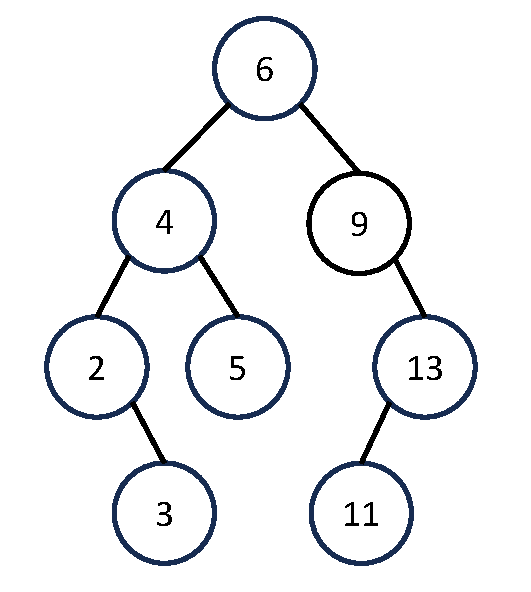
\includegraphics[width=.5\textwidth]{Chapter_2/figures/example_bst.pdf}
    \caption{A simple example of a binary search tree over the set of labels $S
    = \{2,3,4,5,6,9,11,13\}.$}
    \label{example_bst}
\end{figure}

\begin{remark}
    Each node $i$ in a binary search tree can have an associated non-negative
    number called access frequency (or weight, size, probability) $w_i$.
\end{remark}

To construct an optimal binary search tree, that is one with a minimal weighted
path length, we can use Huffman coding.

\begin{definition}[Huffman coding, \citet{huffman_method_1952}]
    Let $A = (\alpha_1, \dots, \alpha_n)$ be a tuple of non-negative numbers.
    To construct an optimal binary tree on $n$ leaves with sizes given by $A$
    we choose the two smallest ones, w.l.g. $\alpha_1$ and $\alpha_2$, and
    join them in a cherry, so that their parent node has size $\alpha_1 + \alpha_2$.
    We now have $A' = (\alpha_1 + \alpha_2, \alpha_3, \dots, \alpha_n)$ as our
    set of $n-1$ nodes. By repeating this procedure until we have only one node
    left, an optimal binary search tree is obtained.
\end{definition}

\begin{proposition}
    The Huffman method maximises $J^1$ on bifurcating trees for a given set of node sizes.
\end{proposition}

\begin{proof}
    By corollary \ref{j1_lower_bound_cor}, the Huffman method maximises $J^1$
    as it minimises the weighted path length.
\end{proof}

As Huffman coding is an optimisation algorithm, $J^1$ can be used to measure how
close a tree constructed using a given set of node sizes is to the maximally
balanced binary tree on the same set. This means we can quantify how close an
alternative algorithm which runs in a faster time complexity, such as arithmetic
coding \citep{pasco_source_1977}, gets to the optimal solution.

\subsection{Expected value of $J^1$ under simple evolutionary processes}\label{expsection}

For applications in evolutionary biology, an important property of balance
indices is their expected value under an evolutionary process. This quantity
helps us compare the trees generated under a null model to the observed data,
and is a valuable part of inferring the underlying evolutionary properties.
Two of the simplest, and most widely studied, processes of tree generation are
the uniform model \citep{rosen_vicariant_1978} and the Yule model
\citep{yule_iimathematical_1925}, which generate bifurcating trees and are
useful null models in evolutionary biology. The Yule model, also known as the
pure birth or coalescent model, is used when considering speciation rates and
patterns \citep{aldous_stochastic_2001, steel_properties_2001}. The uniform
model is used as a null model for comparing neutral evolutionary patterns
against ones which include more complex biological mechanisms
\citep{mooers_inferring_1997, mckenzie_distributions_2000}. While in section
\ref{compscisec} I discussed the static calculation of a balance index for a
given tree, I am also interested in how balanced binary search trees generated
under some stochastic process are. The Yule model is also useful for these
considerations as it is connected to the BST martingale, a statistical tool
used to analyze and predict the behavior of binary search trees, via $L_1$
convergence \citep{chauvin_connecting_2004}. From here, one can extend the
discussion to AVL and red-black trees in a similar way to more complex
evolutionary processes as self-balancing trees will by definition have higher
expected values of $J^1$ than those generated under the Yule process. \par
The expected value of a few indices, and even some higher moments in certain
cases, are known for both Yule and uniform models
\citep{mir_new_2013, m_coronado_sackins_2020, goh_two_2022}. Among these is the
Sackin index, which is particularly useful for our purposes. \par

\begin{definition}[Yule model, \citet{yule_iimathematical_1925}]\label{yuledef}
    Consider a bifurcating tree $T$ on $n$ leaves. To obtain the probability of
    generating $T$ under the Yule model, start with a single node and replace it
    with a cherry. Then, at each step, choose one leaf uniformly at random and
    replace it with a cherry, until the tree has $n$ leaves (figure
    \ref{yule-unif-figure}A). The sum of probabilities of generating $T$ in all
    possible ways is the probability of generating $T$ under the Yule model.
\end{definition}

\begin{definition}[Uniform model, \citet{rosen_vicariant_1978}]\label{unifdef}
    Under the \textbf{uniform model} of tree generation, every bifurcating tree
    on $n$ leaves has an equal probability of being generated, which is equal to
    $n\binom{2n-2}{n-1}^{-1}$ (figure \ref{yule-unif-figure}B).
\end{definition}

\begin{remark}
    We only consider leafy trees with equal leaf sizes generated by the
    processes in definitions \ref{yuledef} and \ref{unifdef}.
\end{remark}

\begin{remark}
    We calculated the exact values of the expectation of $J^1$ under both the
    Yule and uniform models semi-manually by creating all possible $(n+1)$-leaf
    trees given a set of $n$-leaf trees, eliminating duplicates and assigning
    appropriate probabilities in the Yule case, and thus computing the exact
    value of the expectation. The process is inefficient for large trees, and
    we limited our search to $n\leq 11$, the exact and approximate expected
    values for which are found in table \ref{table_values}.
\end{remark}

\begin{figure}[h!]
    \centering
    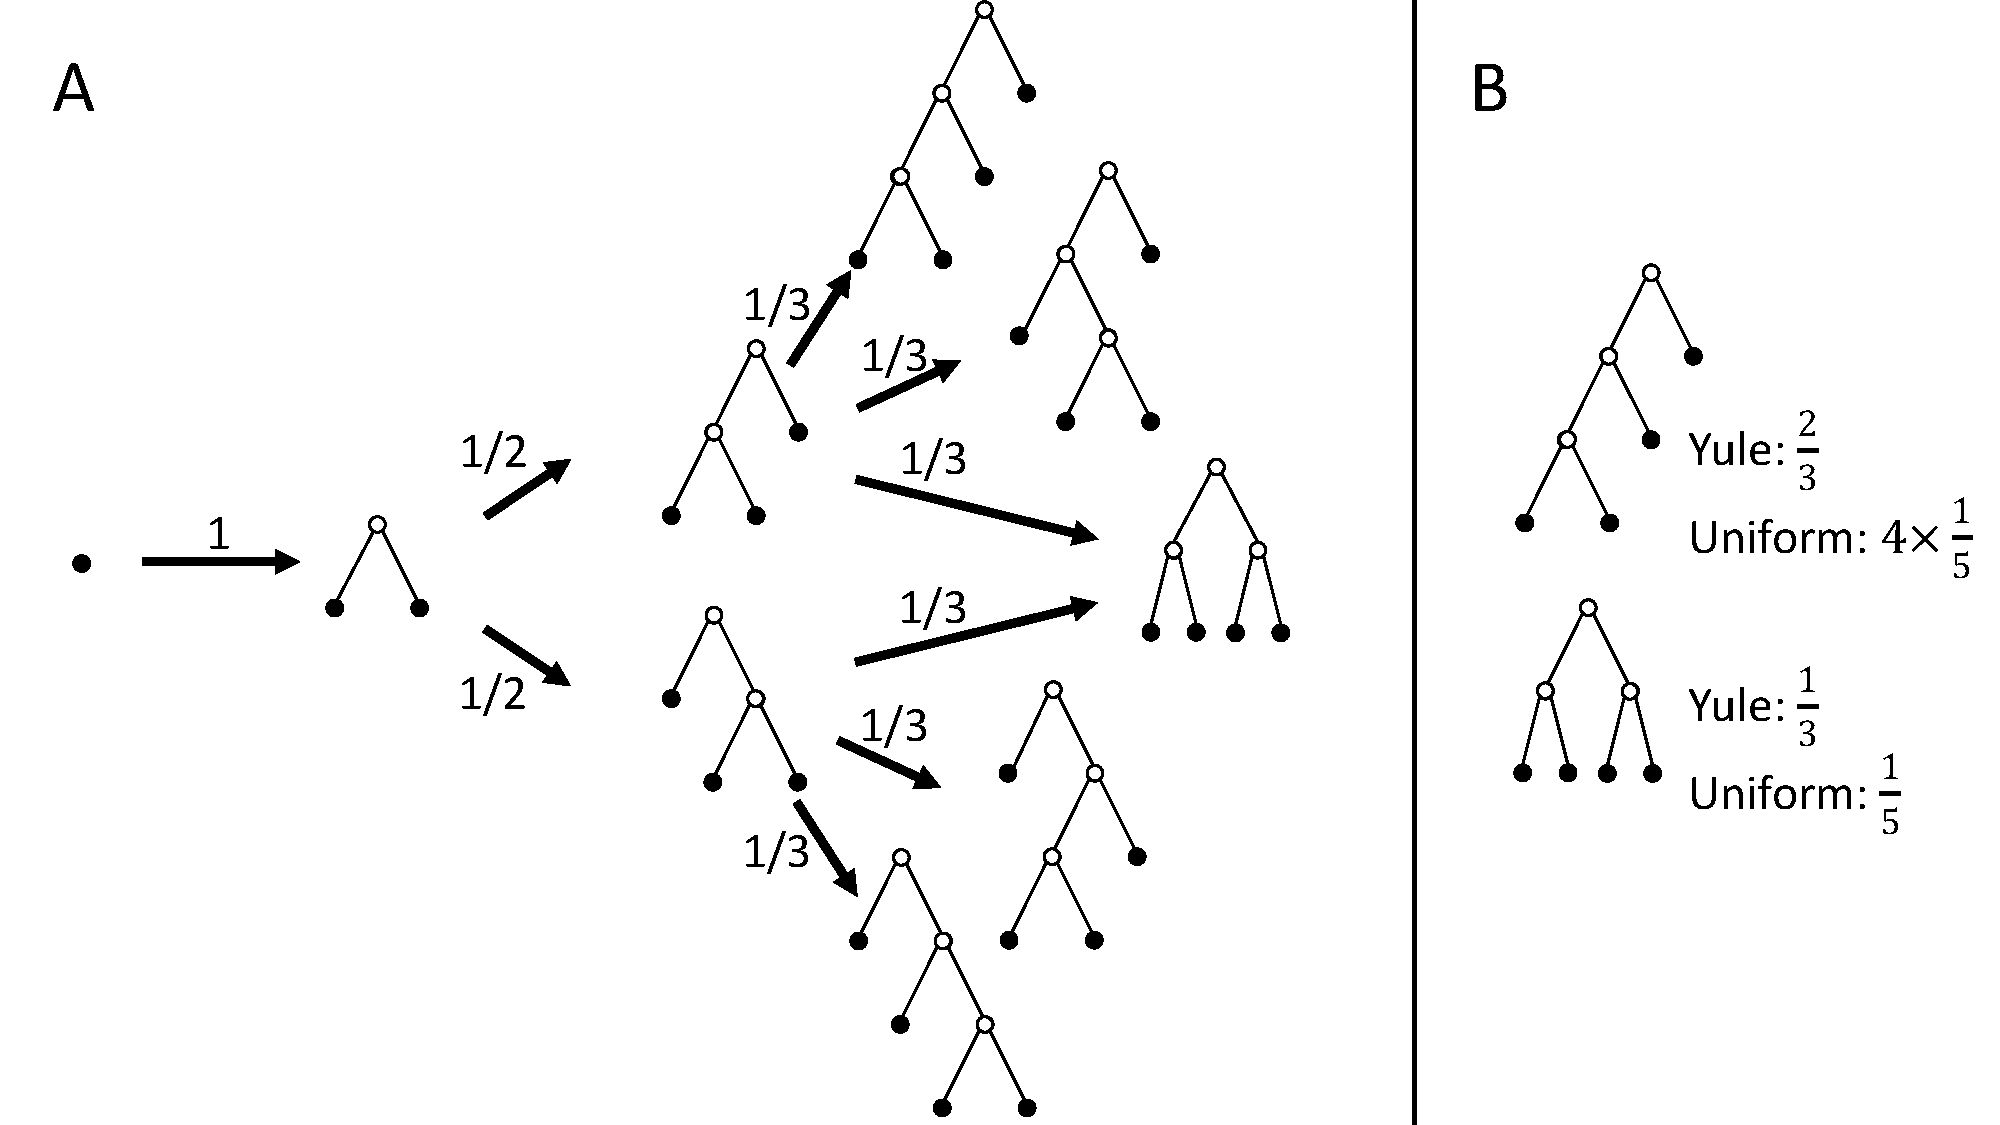
\includegraphics[width=\textwidth]{Chapter_2/figures/yule-unif-figure.pdf}
    \caption{Comparison of probabilities for generation of trees on $4$ leaves
    under the Yule and uniform models. \textbf{A:} Arrows show generation under
    the Yule model. Each of the trees shown on $4$ leaves has the same
    probability under the uniform model. \textbf{B:} Comparison of probabilities
    of tree topologies on $4$ leaves under the Yule and uniform models.}
    \label{yule-unif-figure}
\end{figure}

Under the Yule model, the expected value of the Sackin index for trees on $n$
leaves is
\begin{equation}
    \mathbb{E}_Y^n(I_S) = 2n\sum_{i=2}^n \frac{1}{i},
\end{equation}
as shown in \citet{kirkpatrick_searching_1993}. Equation \eqref{prop6} implies
then that the expected value of $J^1$ for a tree on $n$ leaves is
\begin{equation}
    \mathbb{E}_Y^n(J^1) = \mathbb{E}_Y^n(\frac{n\log_2 n}{I_S}) = n\log_2 n
    \mathbb{E}_Y^n(1/I_S),
\end{equation}
where $\mathbb{E}_Y^n(1/I_S)$ is the harmonic mean of the Sackin index.
The harmonic mean under the Yule process is not a standard result in literature,
nor have I been able to obtain a closed-form solution for this problem so far.
It is possible, however, to compare the harmonic and arithmetic means of $I_S$ by
considering the Jensen gap
\begin{equation}\label{JensenGap}
    \mathcal{J}(f, X) = \mathbb{E}[f(X)] - f(\mathbb{E}[X]),
\end{equation}
with $f(x) = 1/x$.

\begin{theorem}[\citet{liao_sharpening_2017}]\label{jensen_thm}
    Let $X$ be a one-dimensional random variable with mean $\mu$, and
    $P(X\in(a,b))=1$, where $\infty\leq a<b\leq \infty$. If $f(x)$ is a twice
    differentiable function on $(a,b)$, and
    \begin{equation}
        h(x;\nu) = \frac{f(x)-f(\nu)}{(x-\nu)^2} - \frac{f'(\nu)}{x-\nu},
    \end{equation}
    then
    \begin{equation}
        \inf_{x\in(a,b)}\{h(x;\mu)\}\mathrm{Var}(X) \leq \mathbb{E}[f(X)] -
        f(\mathbb{E}[X]) \leq \sup_{x\in(a,b)}\{ h(x;\mu) \}\mathrm{Var}(X).
    \end{equation}
\end{theorem}

\begin{proposition}\label{jensen_prop}
    Let $\mathbb{E}_Y(J^1)$ and $\mathbb{E}_U(J^1)$ be expectation values of
    $J^1$ under the Yule and uniform models respectively. Then:
    \begin{enumerate}[(i)]
        \item $\mathbb{E}_Y(J^1)\to\frac{n\log_2n}{\mathbb{E}_Y(I_S)}$,
        \item $\mathbb{E}_U(J^1)-\frac{n\log_2n}{\mathbb{E}_U(I_S)}$ is bounded
            from both sides,
    \end{enumerate}
    as $n\to\infty$.
\end{proposition}
\begin{proof}
    \textit{(i)} Let $\mu_Y$ be the expected value of the Sackin index under the
    Yule process for trees on $n$ leaves, and $f(x)=\frac{1}{x}$. By theorem
    \ref{jensen_thm}
    \begin{equation}\label{hxmuY}
        h(x;\mu_Y) = \frac{f(x)-f(\mu_Y)}{(x-\mu_Y)^2} - \frac{f'(\mu_Y)}
        {x-\mu_Y} = \frac{1}{x\mu_Y^2}.
    \end{equation}
    We can then substitute this into the inequality given in the theorem
    \begin{equation}\label{JensenApp}
        \frac{n\log_2n}{\frac{(n-1)(n+2)}{2}\mu_Y^2} \text{Var}_Y(I_S) \leq
        \mathbb{E}[J^1] - \frac{n\log_2n}{\mathbb{E}[I_S]} \leq \frac{n\log_2n}
        {\mu_Y^2n\log_2n}\text{Var}_Y(I_S),
    \end{equation}
    where the supremum and infimum of $h(x,\mu)$ are substituted with extremal
    values of the Sackin index on bifurcating trees
    \citep{fischer_extremal_2021}. The expectation of the Sackin index under the
    Yule process is given in equation \eqref{yule_exp_sackin}, and its variance
    is calculated as \citep{cardona_exact_2012}
    \begin{equation}\label{yulevarIS}
        \text{Var}_Y(I_S) = 7n^2 - 4n^2\sum_{i=1}^n\frac{1}{i^2} - 2n
        \sum_{i=1}^{n}\frac{1}{i} - n.
    \end{equation}
    Substituting these expressions into equation \eqref{JensenApp}, we find
    limits
    \begin{align*}
        \frac{n\log_2n}{\frac{(n-1)(n+2)}{2}\mu_Y^2} \text{Var}_Y(I_S) &
        \stackrel{n\to\infty}{\sim} \frac{\log n\left(7n^2 - 4n^2\sum_{i=2}^n
        \frac{1}{i^2}-2n\sum_{i=2}^n\frac{1}{i}-n\right)}{4n^3\left(\sum_{i=2}^n
        \frac{1}{i}\right)^2} \\
        &\sim \frac{\log n}{n} \to 0
    \end{align*}
    for the lower bound on the gap, and
    \begin{align*}
        \frac{n\log_2n}{\mu_Y^2n\log_2n}\text{Var}_Y(I_S) & = \frac{7n^2 - 4n^2
        \sum_{i=2}^n\frac{1}{i^2}-2n\sum_{i=2}^n\frac{1}{i}-n}{4n^2\left(
        \sum_{i=2}^n\frac{1}{i}\right)^2} \\
        & \stackrel{n\to\infty}{\sim} \frac{1}{\left(\sum_{i=2}^n\frac{1}{i}
        \right)^2} \to 0
    \end{align*}
    for the upper bound on the gap. The upper bound reaches a maximum at $n=13$
    and is approximately $0.008$, while the lower bound reaches a maximum at
    $n=8$ and is approximately $0.005$.\\
    \textit{(ii)} Let $\mu_U$ be the expected value of the Sackin's index under
    the uniform model for trees on $n$ leaves, and $f(x)=\frac{1}{x}$. By
    theorem \ref{jensen_thm}
    \begin{equation}\label{hxmuU}
        h(x;\mu_U) = \frac{f(x)-f(\mu_U)}{(x-\mu_U)^2} - \frac{f'(\mu_U)}
        {x-\mu_U} = \frac{1}{x\mu_U^2}.
    \end{equation}
    We can then substitute this into the inequality given in the theorem as in
    \begin{equation}\label{JensenAppU}
        \frac{n\log_2n}{\frac{(n-1)(n+2)}{2}\mu_U^2} \text{Var}_U(I_S) \leq
        \mathbb{E}[J^1] - \frac{n\log_2n}{\mathbb{E}[I_S]} \leq \frac{n\log_2n}
        {\mu_U^2n\log_2n}\text{Var}_U(I_S),
    \end{equation}
    analogously to \eqref{JensenApp}. The expectation of Sackin's index under
    the uniform model is given by \citep{cardona_exact_2012}
    \begin{equation}\label{yule_exp_sackin}
        \mathbb{E}_U(I_S) = \frac{4^{n-1}n!(n-1)!}{(2n-2)!}-n,
    \end{equation}
    and its variance is
    \begin{equation}\label{unifvarIS}
        \text{Var}_U(I_S) = n\frac{10n^2 - 3n - 1}{3} - \frac{(n+1)(n+2)}{2}
        \frac{(2n-2)!!}{(2n-3)!!}-n^2\left(\frac{(2n-2)!!}{(2n-3)!!}\right)^2.
    \end{equation}
    For the limit $n\to\infty$ we can use Stirling's approximation
    \begin{align}
        n! \stackrel{n\to\infty}{\sim} & \sqrt{2\pi n}\left(\frac{n}{e}\right)^n
        \label{stirling}\\
        n!! \stackrel{n\to\infty}{\sim} &
        \begin{cases}
            \sqrt{\pi n}\left(\frac{n}{e}\right)^{n/2},&\text{\quad $n$ even,}\\
            \sqrt{2n}\left(\frac{n}{e}\right)^{n/2}, &\text{\quad $n$ odd,}
        \end{cases}
    \end{align}
    to obtain asymptotic behaviour of the expected value and variance of $I_S$
    under the uniform model. The expectation reduces to
    \begin{align*}
        \mathbb{E}_U(I_S)\stackrel{n\to\infty}{\sim}& \frac{4^{n-1}\sqrt{2\pi n}
        \left(\frac{n}{e}\right)^n \sqrt{2\pi (n-1)}\left(\frac{n-1}{e}
        \right)^{n-1}}{\sqrt{2\pi (2n-2)}\left( \frac{2n-2}{e} \right)^{2n-2}}
        - n \\
        \sim & \frac{\sqrt{\pi n}n^n}{e(n-1)^{n-1}}-n\\
        \sim & \sqrt{\pi} \exp\left[ (n+\frac{1}{2})\log n - (n-1)\log(n-1)
        \right] - n\\
        \sim & \sqrt{\pi} n^{\frac{3}{2}} - n
    \end{align*}
    and the variance
    \begin{align*}
        & \text{Var}_U(I_S)  \stackrel{n\to\infty}{\sim}  \frac{10}{3}n^3 - n^2
        - \frac{1}{3}n - \frac{n^2 + 3n +2}{2}\frac{\sqrt{\pi (2n-2)}\left(
        \frac{2n-2}{e}^{n-1} \right)}{\sqrt{2 (2n-3)}\left( \frac{2n-3}{e}^{n-1/2}
        \right)}\\
        &-  n^2\left( \frac{\sqrt{\pi (2n-2)}\left( \frac{2n-2}{e}^{n-1} \right)}
        {\sqrt{2 (2n-3)}\left( \frac{2n-3}{e}^{n-1/2} \right)} \right)^2\\
        \sim & \frac{10}{3}n^3 - n^2 - \frac{1}{3}n - \frac{n^2+3n+2}{2}
        \sqrt{\frac{e\pi}{2}}\exp\left[(n-1)\log\frac{2n-2}{2n-3}+
        \frac{1}{2}\log(2n-3)\right] \\
        &- n^2\exp\left[ \log(2n-3) \right]\\
        \sim & \frac{4}{3}n^3 + 2n^2 - \frac{1}{3}n - \frac{n^\frac{5}{2}+
        3n^\frac{3}{2}+2n^\frac{1}{2}}{2}\sqrt{e\pi}.
    \end{align*}
\end{proof}

\begin{figure}[h]
    \centering
    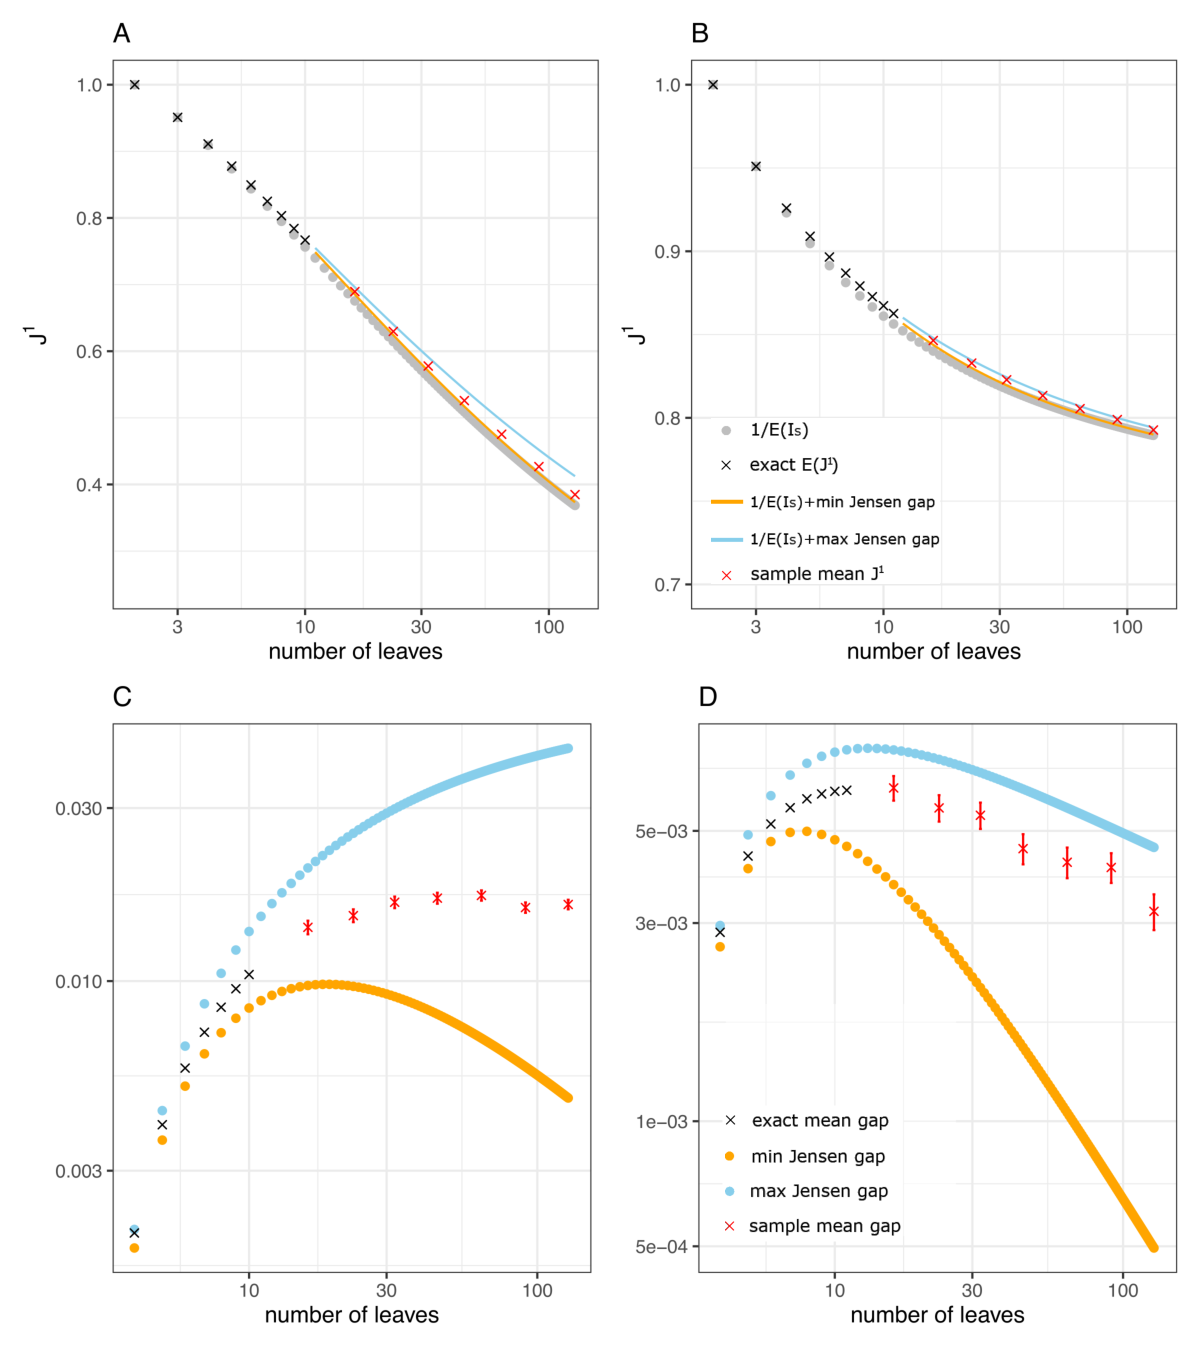
\includegraphics[width=\textwidth]{Chapter_2/figures/jensen_plots_final_edited.pdf}
    \caption{\textbf{Top row}: True values of $\mathbb E(J^1)$ for up to $10$
    leaves were calculated manually, and the approximations up to $128$ leaves
    were calculated as $n\log_2n/\mathbb E(I_S)$. \textbf{A} --- uniform model,
    \textbf{B} --- Yule model.\\
    \textbf{Bottom row}: The Jensen gap of $\mathbb{E}(J^1)$ calculated for
    trees up to $128$ leaves under the uniform model (\textbf{C}), and the Yule
    model (\textbf{D}). The size of the gap is calculated as the difference
    between the true and approximate expected value, with the gaps for $2$ and
    $3$ leaves equal to zero as there is only one possible bifurcating tree
    shape for each of those values. Refer to table \ref{table_values} for
    numerical values of the gap size for the first several values of $n$.
    The red crosses in \textbf{A} and \textbf{B} represent sample mean $J^1$
    values for $100000$ trees generated under the uniform model and Yule
    process, and the difference between the approximate gap size and the sample
    mean, with standard error represented by error bars, in \textbf{C} and
    \textbf{D}.}
    \label{jensenfig}
\end{figure}
\begin{figure}[h]
    \centering
    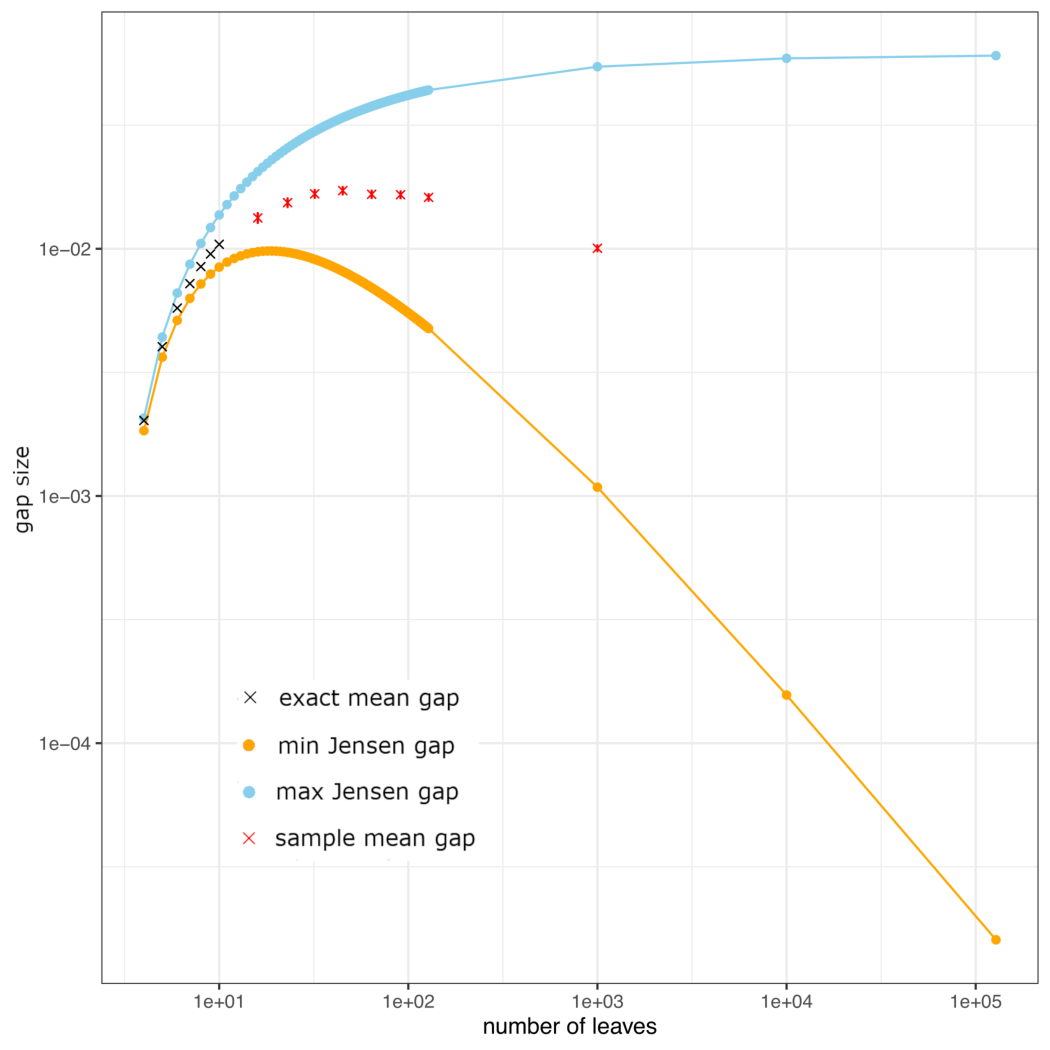
\includegraphics[width=\textwidth]{Chapter_2/figures/jensen_gap_1k.pdf}
    \caption{The convergence of the upper bound to $4/3\pi$ is much slower than
    the convergence of the lower bound to $0$, and the maximum it reaches over
    the plotted range is $0.0604$ for $n=128000$. The red crosses, as in figure
    \ref{jensenfig}, suggest convergence of the gap size.}
    \label{conv_upper_fig}
\end{figure}
\begin{figure}[h]
    \centering
    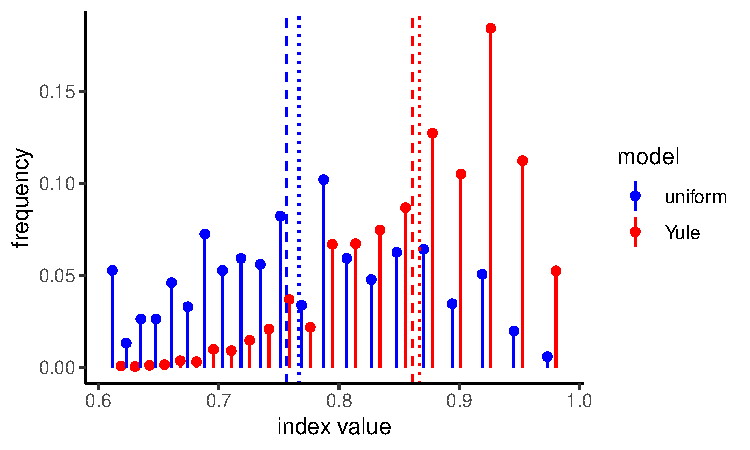
\includegraphics{Chapter_2/figures/var_fig.pdf}
    \caption{Higher variance in the uniform model leads to a non-zero upper
    bound on the Jensen gap. Shown are frequencies of $J^1$ values on $10$-leaf
    trees generated under the Yule and uniform models. The dashed lines
    represent the true expected value of $J^1$, and the dotted lines the
    approximate value calculated as $\frac{n\log_2n}{\mathbb{E}(I_S)}$}.
    \label{var_fig}
\end{figure}
\clearpage

The lower bound of $\mathbb{E}_U(J^1)-\frac{n\log_2n}{\mathbb{E}_U(I_S)}$ goes
to $0$ as $\frac{\log n}{n}$, while the upper bound tends to $\frac{4}{3\pi}$
for $n\to\infty$. This is a consequence of high variance in the uniform model
(figure \ref{var_fig}), as each tree on $n$ leaves is selected with equal
probability while the number of trees on $n$ grows exponentially with $n$,
the number of leaves. While I cannot prove analytically that the size of the
Jensen gap in this case tends to $0$, I can generate random trees using the
uniform model and compare the sample mean to the approximation using the
expected value of the Sackin index. In figure \ref{jensenfig}, I show behaviour
of the Jensen gap and its bounds for $J^1$ under the Yule and uniform models.
The red crosses in figures \ref{jensenfig}C and \ref{conv_upper_fig} indicate
that the gap size does converge for $n\to\infty$. Therefore, I propose the
following conjecture:

\begin{conjecture}
    For trees generated under the uniform model on $n\to\infty$ leaves, the
    following holds
    \begin{equation}
        \mathbb{E}_U(J^1) \to \frac{n\log_2n}{\mathbb{E}_U(I_S)}.
        \label{conjecture1}
    \end{equation}
\end{conjecture}

\begin{table}[h]
    \centering
    \begin{tabular}{|c|c|c|c|c|}
        \hline
        $n$ & $n\log_2n/\mathbb{E}_Y(J^1)$ & $\mathbb{E}_Y(I_S)$ & $n\log_2n/
        \mathbb{E}_U(J^1)$ & $\mathbb{E}_U(I_S)$\\
        \hline
        $2$ & $2$ & $2$  & $2$ & $2$ \\
        \hline
        $3$ & $5$ & $5$  & $5$ & $5$ \\
        \hline
        $4$ & $216/25$ & $26/3$ & $360/41$ & $44/5$ \\
        \hline
        $5$ & $728/57$ & $77/6$ & $3822/289$ & $99/7$ \\
        \hline
        $6$ & $1162800/67217$ & $87/5$ & $18.25643$ & $386/21$ \\
        \hline
        $7$ & $199806750/9017743$ & $223/10$ & $23.81979$ & $793/33$ \\
        \hline
        $8$ & $27.29901$ & $962/35$& $29.87282$ & $12952/492$\\
        \hline
        $9$ & $32.68993$ & $4609/140$ & $36.38201$ & $26333/715$ \\
        \hline
        $10$ & $38.30246$ & $4861/126$ & $43.31989$ & $106762/2431$ \\
        \hline
        $11$ & $44.11464$ & $55991/1260$ & n/a & n/a \\
        \hline
    \end{tabular}
    \caption{Comparison of exact and approximate expected values of $J^1$ and
    $I_S$ under the Yule and uniform models.}
    \label{table_values}
\end{table}

\subsection{Analytic properties of the $J^1$ index}
The index $J^1$ is normalised in a way which makes comparison of its values on
trees of different sizes valid \citep{lemant_robust_2022}. As $J^1$ was defined
to take into account node sizes, it can take any value between $0$ and $1$ for
any given tree topology (figure \ref{balcat}). Furthermore, since $J^1$ is
defined to be $0$ on linear trees, finding its minimal value on a given number
of nodes is trivial. In this section I investigate extremal values on trees
where I impose restrictions to both topology and node size distributions, i.e.
consider only leafy trees with out-degree of each internal node greater than $1$.

\begin{figure}[h]
    \centering
    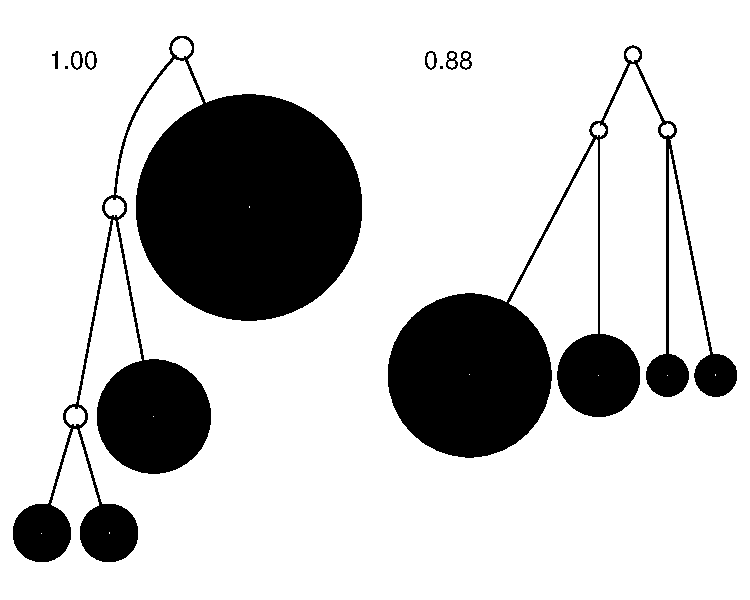
\includegraphics[width=0.8\textwidth]{Chapter_2/figures/balcat.pdf}
    \caption{By including the node-balance function $W^1$ in $J^1$, we allow for
    the possibility of perfectly balanced caterpillars (left) and less balanced
    fully symmetric trees (right) based on the node size distribution in the
    tree. The leaf sizes in these two trees are identical, with a ratio
    $4:2:1:1$ from largest to smallest.}
    \label{balcat}
\end{figure}

\subsection{Properties of $J^1$ on different tree families}

For most balance indices in use in evolutionary biology, the least balanced tree
for a given number of leaves $n$ is the binary caterpillar tree. I have
previously derived a general expression for leafy trees of this topology
\citep{lemant_robust_2022}
\begin{equation}
    J^1(T_C) = \frac{2n\log_2n}{(n-1)(n+2)}.\label{caterpillar}
\end{equation}
Most balance indices in literature define the caterpillar topology as the least
balanced one \citep{fischer_tree_2021}. Intuitively, this makes sense as balance
is often associated with symmetry, and the caterpillar is the most asymmetric
bifurcating tree. However, in the context of the $J^1$ index, tree topology is
just one of a few factors which contribute to the balance score of a tree,
especially since the index does not limit the space of trees to bifurcating ones.
Also important to consider are node sizes and, more specifically, how the population
is split across different subtrees in the tree of interest. Let us consider a
slightly altered caterpillar topology. \par

\begin{figure}[h]
    \centering
    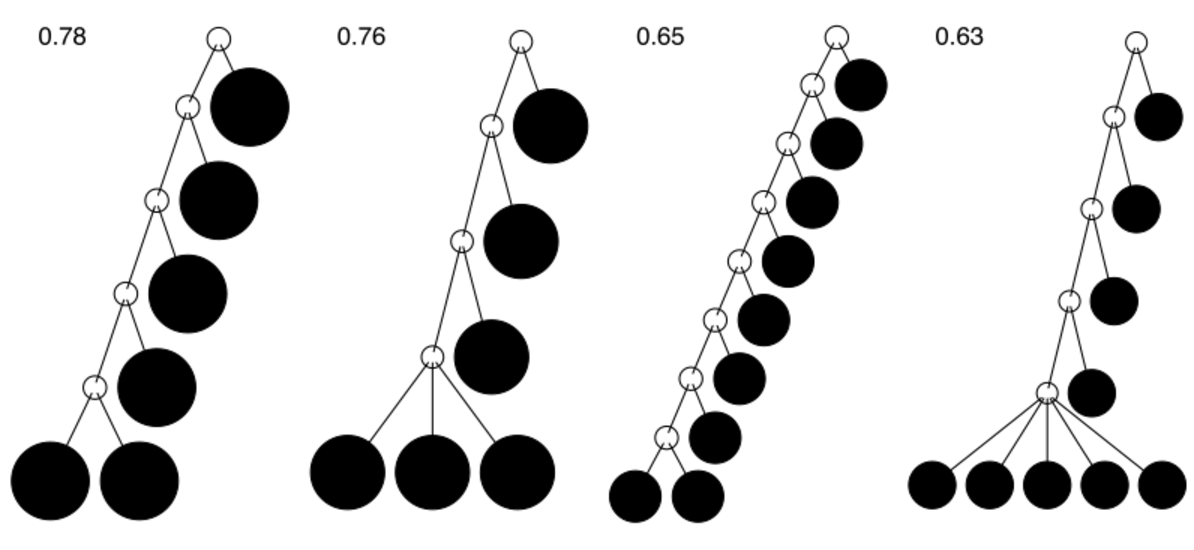
\includegraphics[width=\textwidth]{Chapter_2/figures/example_figure_1.pdf}
    \caption{If we limit our search to leafy trees with equal leaf sizes, the
    least balanced tree on a given number of leaves is not necessarily the
    caterpillar. Pictured are the caterpillar trees on $6$ and $9$ leaves, as
    well as minimally balanced brooms for $6$ and $9$ leaves,
    with corresponding $J^1$ values.}
    \label{example_figure_1}
\end{figure}

\begin{definition}
    Let $T_B$ be a leafy tree on $n$ leaves. Let every internal node of $T_B$
    except for the most distant one from the root have out-degree $2$ such that
    one of its descendants is a leaf, and the other an internal node. Further,
    let the internal node most distant from the root have out-degree $k$.
    Then we call tree $T_B$ a \textbf{broom tree}.\\
    We call the leaves attached to the internal node with the highest out-degree
    the \textbf{broom head}, and the remaining leaves are attached to the \textbf{handle}.
\end{definition}
A general expression of $J^1$ for this family of trees is then derived.
\begin{proposition}\label{broom_prop}
    The value of $J^1$ for a broom tree $T_B$ on $n$ leaves, of which $k$ in the broom head is
    \begin{equation}
        J^1(T_B) = \frac{2\left( n \log_2 n - k \log_2 k + k \right)}{(n+k)(n-k+1)}.\label{J1Tb}
    \end{equation}
\end{proposition}
\begin{proof}
    \begin{align*}
        J^1(T_B) &= \frac{1}{\sum_{l=k}^{n}l} \sum_{i\in\tilde{V}} S_i^{*}
        \sum_{j\in C(i)}W_{ij}^{1}\\
        &= \frac{-2}{(n+k)(n-k+1)}\sum_{i \in \tilde{V}} S_i^*\sum_{j\in C(i)}
        \frac{S_j}{S_i^*}\log_{d^+(i)} \frac{S_j}{S_i^*}\\
        &=\frac{-2}{(n+k)(n-k+1)}\left(\sum_{\substack{i \in \tilde{V}\\d^+(i)=2}}
        S_i^*\sum_{j\in C(i)} \frac{S_j}{S_i^*}\log_2\frac{S_j}{S_i^*}+k\cdot
        k\cdot\frac{1}{k}\log_k \frac{1}{k}\right)\\
        &= \frac{-2}{(n+k)(n-k+1)}\left(\sum_{\substack{i \in \tilde{V}\\d^+
        (i)=2}} S_i\left(\frac{S_i-1}{S_i}\log_2\frac{S_i-1}{S_i}+\frac{1}{S_i}
        \log_2\frac{1}{S_i}\right)-k\right)\\
        &= \frac{2}{(n+k)(n-k+1)}\left( \sum_{i=k+1}^{n} i\left( \frac{i-1}{i}
        \log_2\frac{i}{i-1}+\frac{1}{i}\log_2 i \right)+k \right)\\
        &= \frac{2}{(n+k)(n-k+1)}\left(  \sum_{i=k+1}^{n}\left( (i-1)\log_2
        \frac{i}{i-1}+\log_2 i \right) +k \right)\\
        &= \frac{2}{(n+k)(n-k+1)}\left( log_2\frac{n^n k!}{k^k n!}+\log_2
        \frac{n!}{k!}+k \right)\\
        &= \frac{2}{(n+k)(n-k+1)}\left( \log_2\frac{n^n}{k^k}+k \right)\\
        &= \frac{2}{(n+k)(n-k+1)}\left( n \log_2 n - k \log_2 k + k \right)
    \end{align*}
\end{proof}

The result of proposition \ref{broom_prop} is directly generalisable in the
following way.

\begin{proposition}\label{q-broom-prop}
    For a broom tree $T_{Bq}$ on $n$ leaves, of which $k$ in the broom head,
    such that the sizes of leaves in the head sum to $q\in \mathbb R$, and the
    leaves in the handle all of equal size $1$, the value of $J^1$ is
    \begin{align*}
        J^1(T_{Bq}) &= \frac{1}{(n-k+1)(q+(n-k)/2)}\\
        &\times\left( q\log_k q-\left(\sum_{i=1}^{k}l_i\log_k l_i\right)+(q+n-k)
        \log_2(q+n-k) - q\log_2q \right),\numberthis\label{J1Tbq}
    \end{align*}
    where $l_1,\dots,l_k$ are the leaf sizes which add up to $q$.
\end{proposition}

In figure \ref{example_figure_1} I show that the caterpillar is not the
minimally balanced leafy tree for a few tree sizes. To take it a step further,
consider the following proposition.

\begin{proposition}\label{cat_prop}
    For leafy trees on $n$ leaves and no linear parts, the caterpillar minimises $J^1$ iff $n<5$.
\end{proposition}

\begin{proof}
    Let $J^1_B(n,k)$ denote the value of $J^1$ on a broom tree with $n$ leaves,
    of which $k$ in the broom head. Then
    \begin{align}
        J^1_B(n,2) = & \frac{2n\log_2n}{(n+2)(n-1)}, \label{j1bn2}\\
        J^1_B(n,3) = & \frac{2}{(n+3)(n-2)}(n\log_2n - 3\log_2 3 + 3).\label{j1bn3}
    \end{align}
    Consider the case when $J^1_B(n,2) < J^1_B(n,3)$. Plugging in equations
    \eqref{j1bn2} and \eqref{j1bn3}, we can rearrange the inequality to find
    \begin{equation}
        8n\log_2n - 6(n^2+n-2)\log_2 3 + 6(n^2+n-2) > 0,
    \end{equation}
    which changes sign at $0, 0.667, 1$ and $4.168$. Setting the first
    derivative of this expression to zero
    \begin{equation*}
        8\log_2n+\frac{8}{\log 2}-(12n+6)\log_2 3 + 12n + 6 = 0
    \end{equation*}
    we find solutions around $n=0.822$ and $n=2.888$, the latter of which
    signifies a local maximum. Therefore, as $n$ can only take positive integer
    values, valid solutions for which the caterpillar is less balanced than the
    broom with $3$ leaves in the broom head according to the index $J^1$ are $3$
    and $4$, with the $k=3$ broom being less balanced otherwise.
\end{proof}

This proposition gives us a threshold for the number of leaves at which the
caterpillar is no longer the minimally balanced tree for the given number of
leaves, which sets $J^1$ apart from conventional balance indices (figure
\ref{Rfigures}A). However, I am yet to prove the following statement.

\begin{conjecture}\label{conj}
    For leafy trees on $n$ leaves and no linear parts, the tree that minimises
    $J^1$ belongs to the broom family.
\end{conjecture}

\subsection{Behaviour as $n\to\infty$}

\begin{figure}[h!]
    \begin{center}
    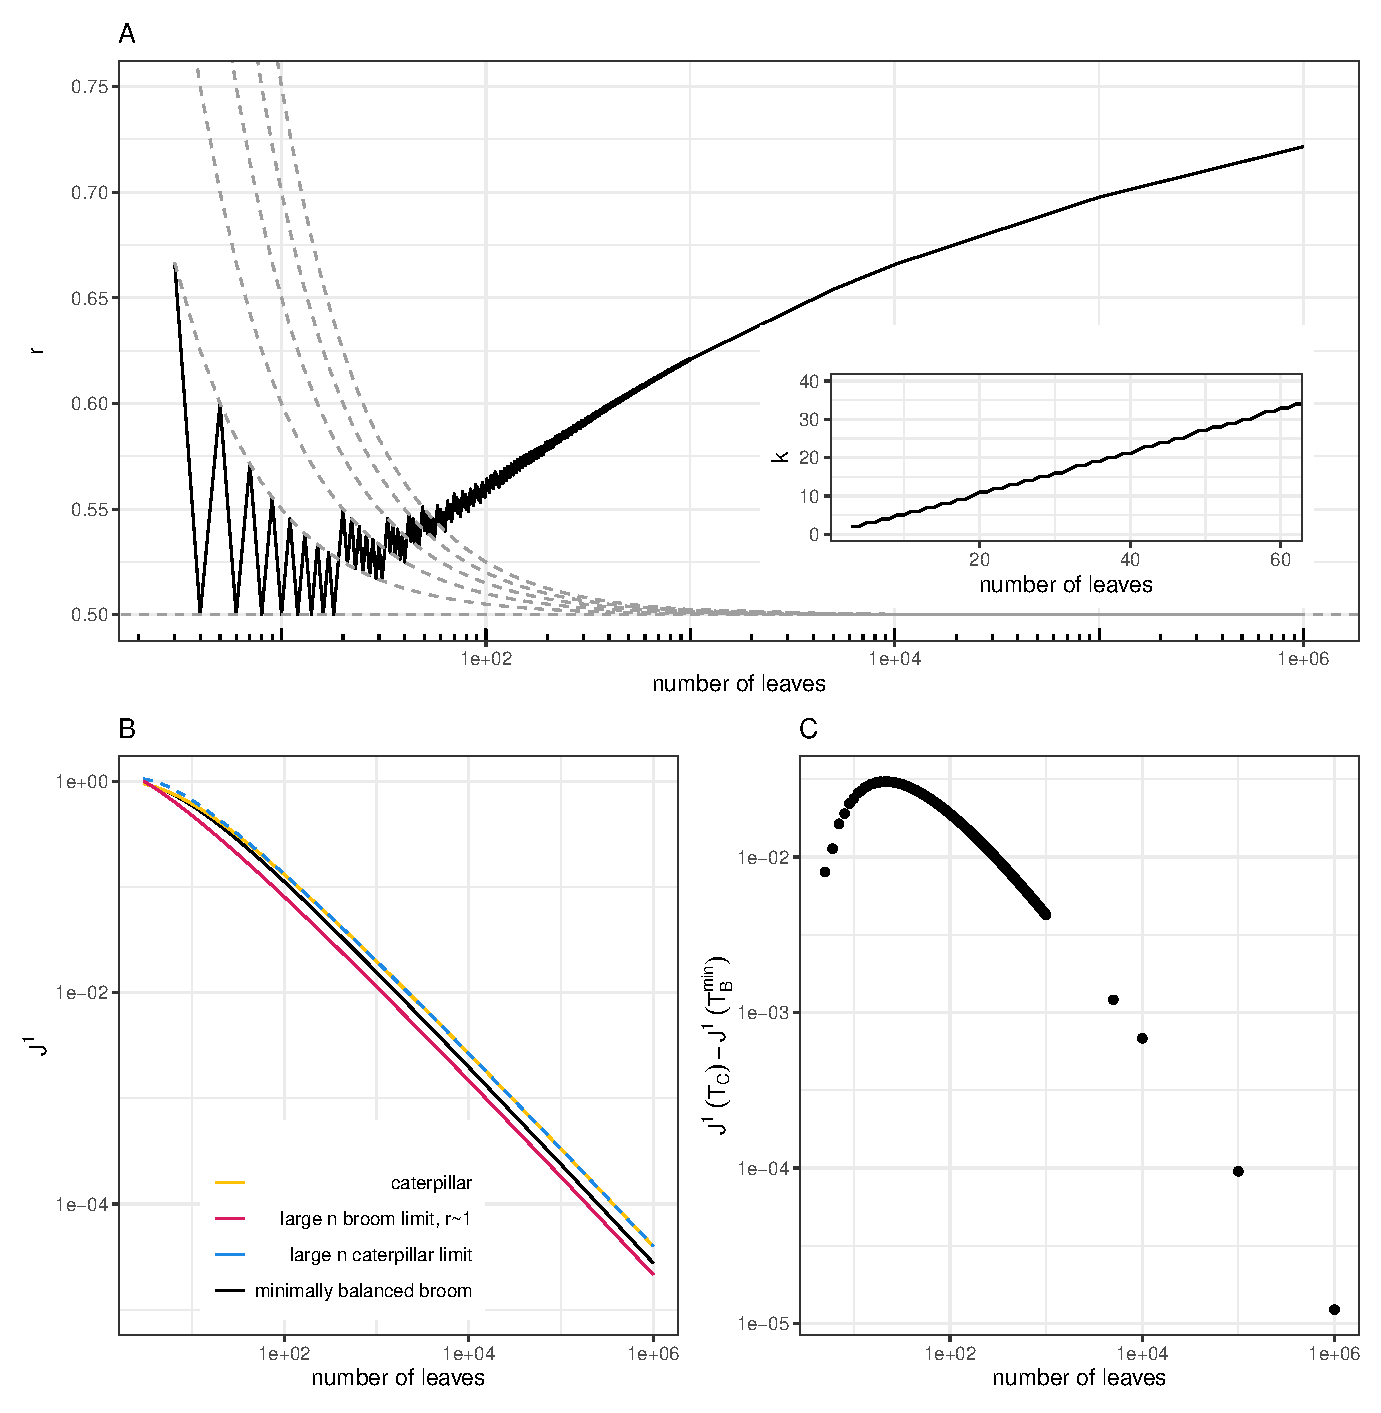
\includegraphics[width = \textwidth]{Chapter_2/figures/j1_figure_3_plots.pdf}
    \caption{The labels used in the figures are as above - $n$ for number of
        leaves, $k$ for number of leaves in the broom head, $r=n/k$.
        \textbf{A:} Value of $r$ for which the minimum value of $J^1$ is
        obtained on leafy trees. Trees on $n$ leaves which satisfy
        $r = \frac{n+a}{2n}$, for $a=0,1,2,\dots$ lie on the dashed grey lines.
        The inset plot shows $k = rn$, the number of leaves attached at the
        broom head. \textbf{B:} Comparison of true and approximate values of
        $J^1$ for the caterpillar and minimally balanced broom trees as a
        function of $n$. \textbf{C:} The difference between values of $J^1$ of
        the minimally balanced broom and the caterpillar trees.}
    \label{Rfigures}
    \end{center}
\end{figure}
\clearpage

I have derived general behaviour of $J^1$ on broom and caterpillar trees for a
given number of leaves $n$, showing that caterpillar trees are not necessarily
minimally balanced for a given number of leaves. If we let $n\to\infty$, the
value of $J^1$ for the caterpillar from equation \eqref{caterpillar} will
behave like
\begin{equation}
    \lim_{n\to\infty} J^1(T_C) = \frac{2\log_2n}{n}. \label{caterpillarlim}
\end{equation}
As $J^1$ is not limited to trees with equal leaf sizes, there is a threshold we
can impose on the broom tree beyond which the caterpillar is less balanced.

\begin{proposition}\label{p-broom-prop}
    Let $T_B(n)$ be a broom tree on $n$ leaves such that the leaves on the
    handle and head have sizes $f$ and $fp$ respectively, and $T_C(n)$ be a
    caterpillar tree on $n$ leaves of equal sizes $f$. Then
    \begin{equation}\label{p-broom-cond}
        J^1(T_B) > J^1(T_C) \text{\quad iff \quad} p<\frac{1}{2},
    \end{equation}
    as $n\to\infty$.
\end{proposition}
\begin{proof}[Proof of proposition \ref{p-broom-prop}]
    Let $n\to\infty$. The the value of $J^1$ for the caterpillar tree tends to
    \begin{equation*}
        J^1(T_C) = \frac{2\log_2n}{n},
    \end{equation*}
    and for the broom tree with equally sized leaves of size $p$ in the broom head
    \begin{equation*}
        J^1(T_{B,p}) = \frac{2}{n(1-r)(1+r(2p-1))}\left[ (r(p-1)+1)\log_2
        n(r(p-1)+1) - rp\log_2 nrp \right].
    \end{equation*}
    We can evaluate the difference between these expressions:
    \begin{align*}
        J^1(T_C) - J^1(T_{B,p})  \sim &  (1-r)(1+r(2p-1))\log_2n+rp\log_2nrp \\
        & - (r(p-1)+1)\log_2n(r(p-1)+1) \\
        \sim & ((1-r)(1+r(2p-1))-(r(p-1)+1)+rp)\log_2n + o(\log_2n).
    \end{align*}
    The difference is dominated by the term containing $\log_2n$ which is always
    positive. The term in the brackets preceding it can be negative, however:
    \begin{equation*}
        (1-r)(1+r(2p-1)) - r(p-1) + 1 + rp = r(1-r)(2p-1).
    \end{equation*}
    As $r = k/n$, with $k$ the number of leaves in the broom head, it is always
    positive. Thus, the expression is negative only when $2p-1<0$ or $p<\frac{1}{2}$
\end{proof}

\begin{figure}[h!]
    \centering
    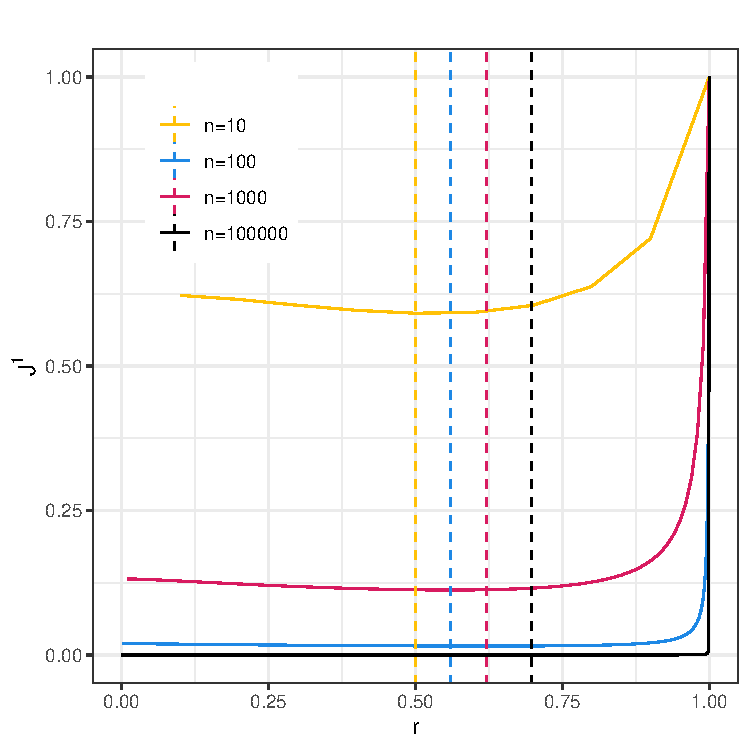
\includegraphics[width=.7\textwidth]{Chapter_2/figures/j1_lines_plot.pdf}
    \caption{Values of $J^1$ on trees of different sizes calculated using
    equation \eqref{J1Tb} for different values of $r=k/n$. The dashed lines are
    at values of $r$ which minimise $J^1$.}
    \label{j1_lines_plot}
\end{figure}

For broom trees, the behaviour is a little more complicated and, perhaps,
counter-intuitive (figure \ref{j1_lines_plot}). Consider the following.

\begin{proposition}\label{ropt_prop}
    Let $\mathcal{T}_B(n)$ be the set of all leafy broom trees with equal leaf
    sizes on $n$ leaves, $r = \frac{k}{n}$ where $k$ is the number of leaves in
    the broom head for a given tree, and $r_\text{opt}$ the value of $r$ which
    minimises $J^1$ for a given $n$. Then $r_\text{opt}\to 1$ as $n\to\infty$.
\end{proposition}
\begin{proof}
    Let $r = k/n$ and $J^1_B(n,r)$ the value of $J^1$ for a broom tree on $n$
    leaves, of which $k$ in the head. Then
    \begin{equation}
        J^1 \stackrel{n\to\infty}{=} \frac{2}{n(1-r)(r+1)}((r+1)\log_2n(r+1)-
        r\log_2nr)
        \label{broomlim}
    \end{equation}
    which is minimised for $r\to1$.
\end{proof}

The proposition says that most leaves on a minimally balanced broom tree will be
concentrated in the head, with comparatively few on the handle, resembling a
star tree more closely than a caterpillar tree. However, one must take into
account how imbalanced the nodes above the broom head are, since one of their
subtrees contains most of the tree's leaves, whereas the other is a single leaf.
For practical purposes, the difference between the $J^1$ values of the minimally
balanced broom and the caterpillar for the number of leaves $n\to\infty$ is
small and decreases rapidly as $n$ grows (figure \ref{Rfigures}B,
\ref{Rfigures}C). \par
Finding the true value of $k$ which minimises $J^1(T_B)$ analytically is
difficult. The derivative with respect to $k$ of equation \eqref{J1Tb} yields a
transcendental equation which is not analytically solvable. I also cannot
analytically determine whether broom trees minimise $J^1$ for a given number of
leaves. However, I have exhaustively checked whether the broom minimises $J^1$ up
to $12$ leaves --- which it does. Beyond that, the number of possible trees
grows too rapidly for a similar verification to be computationally feasible
without an efficient tree generating algorithm for trees with arbitrary node
degree distributions.

\section{Discussion}
The aim of this chapter was to explore deeper analytic properties of the universal
balance index $J^1$ and carve its place in the broader context of tree balance
by extending past results and uncovering new connections. \par
In the chapter I focussed on trees with uniform branch lengths, as $J^1$ was not
defined with them under consideration. A further generalisation of metric
describing tree properties is therefore the logical next step
\citep{noble_new_2023}. \par
I calculated an approximate expectation of $J^1$ under the most common null
models used in evolutionary biology. Having a good approximation for the
expected value of $J^1$ is a crucial result in the development of this index,
as it allows us to employ it in the analysis of evolutionary processes on
phylogenetic trees. The next step in this direction would be to obtain a
closed-form solution for the expectation of $J^1$, as well as its variance.\par
Finally, I only touched upon directly obtainable relationships without
considering different real-world use cases of the index and the implications of
equation \eqref{prop6}. This is another avenue of future research as there may
exist a relationship between the way indices vary with time and the underlying
evolutionary process growing the associated tree.

